\documentclass{beamer}
\usepackage{amsmath}
\usepackage{graphicx}
\usepackage{subfig}
\usepackage{tikz}
\usepackage[style=verbose]{biblatex}

\makeatletter
\let\@@magyar@captionfix\relax
\makeatother

\bibliography{../link.bib}
\renewcommand{\footnotesize}{\tiny}
\title{Latent Variable Machine Learning Algorithms: Applications in a Nuclear Physics Experiment
}
\author{Robert Solli}
\institute{University of Oslo, Expert Analytics AS}
\date{\today}

\begin{document}
\begin{frame}[t]{Masters Presentation}
	\titlepage
\end{frame}

\begin{frame}[t]{Outline}
	\begin{enumerate}
		\item Introducing the Active Target Time Projection Chamber (AT-TPC)
		\item Challenges with traditional analysis of AT-TPC data - and the evangilization of Machine Learning
			\begin{enumerate}[(i)]
				\item Recap of central literature 
				\item Introducing thesis problem statements
			\end{enumerate}
		\item An introduction to central Machine Learning concepts
		\item The Auto-Encoder neural network
		\item Results 
		\item Summary, Conclusion and Outlook
	\end{enumerate}
\end{frame}

\begin{frame}[t]{AT-TPC}
	\begin{figure}
		\centering
		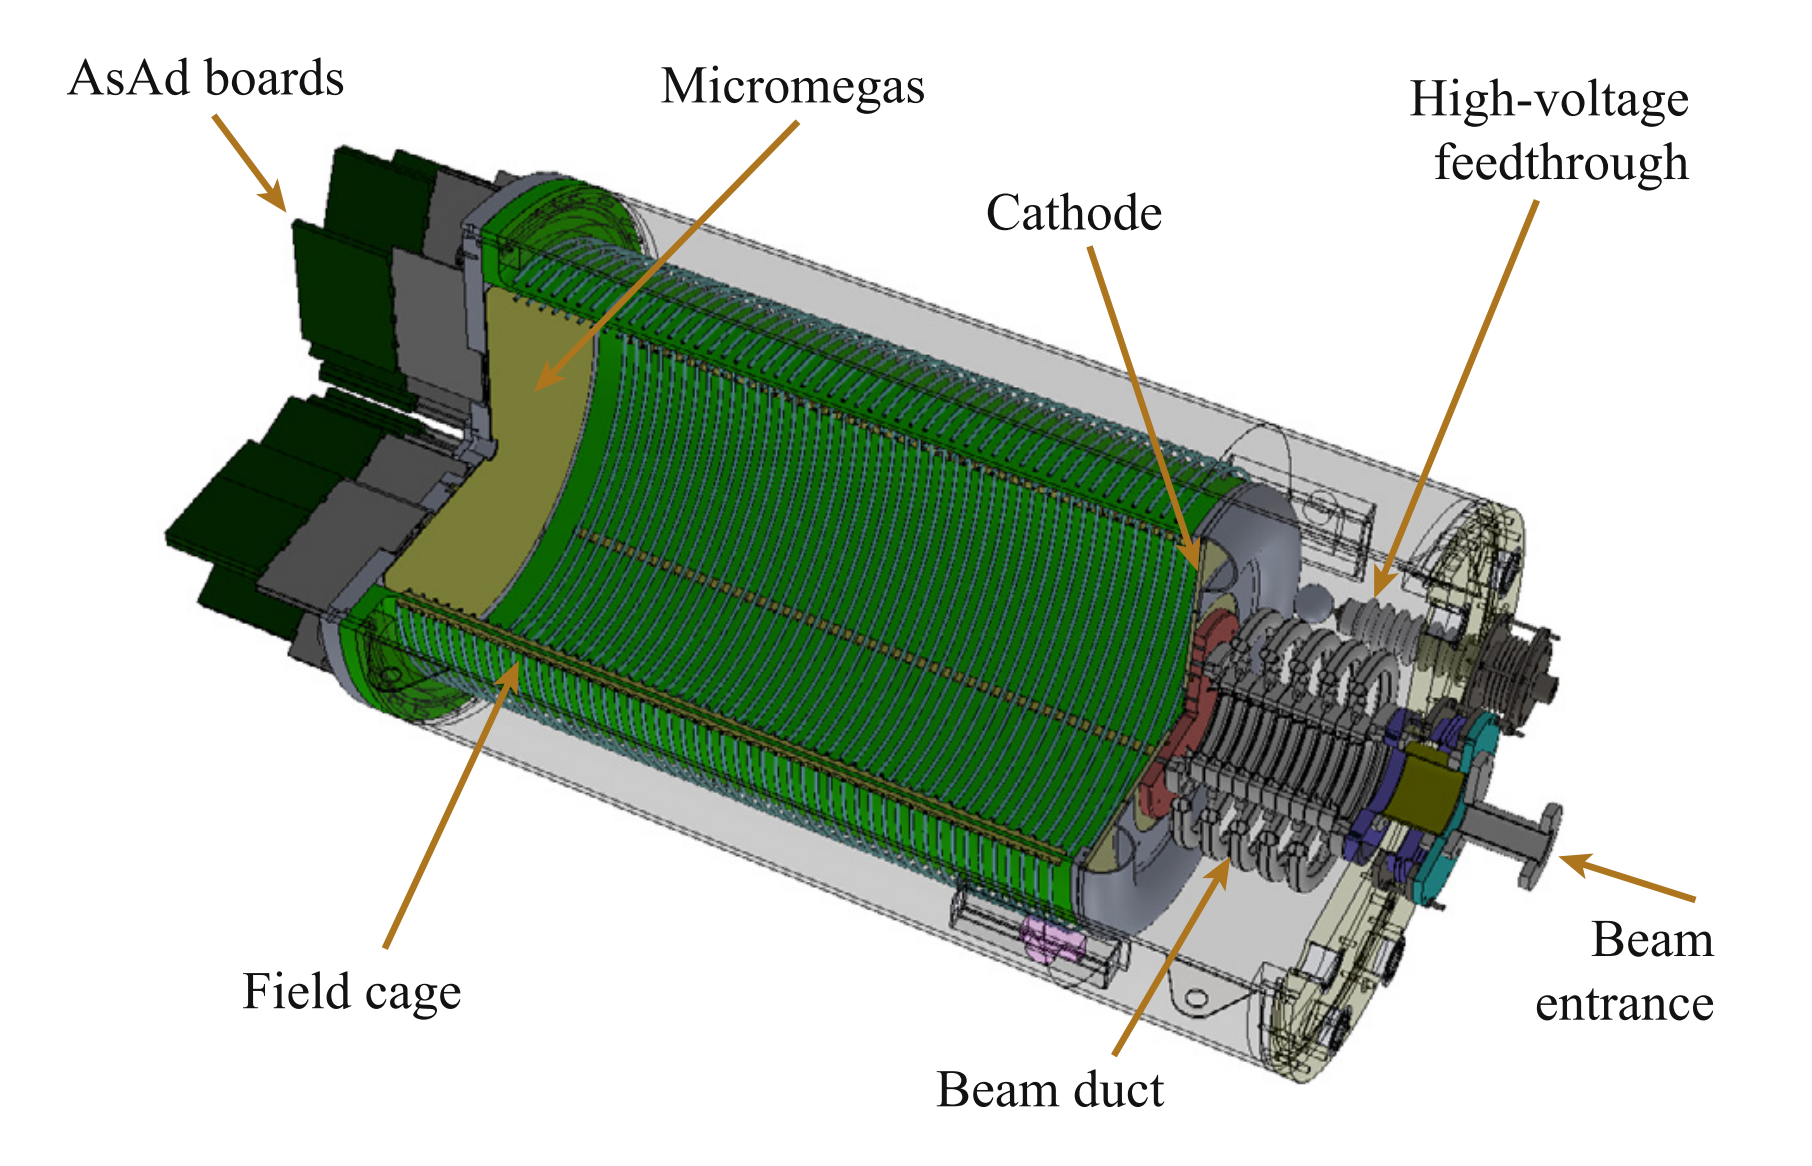
\includegraphics[height=3cm]{../chapters/experimental_background/plots/at_tpc_schematic.png}
		\caption{Diagram of the AT-TPC \footcite{Bradt2017a}}\label{fig:attpc}
	\end{figure}
	The AT-TPC is an experiment set up at the rare isotopes facility on the Michigan State University campus. The AT-TPC is commissioned to capture reactions with exotic nuclei.
\end{frame}

\begin{frame}[t]{AT-TPC}
	\begin{figure}
		\centering
		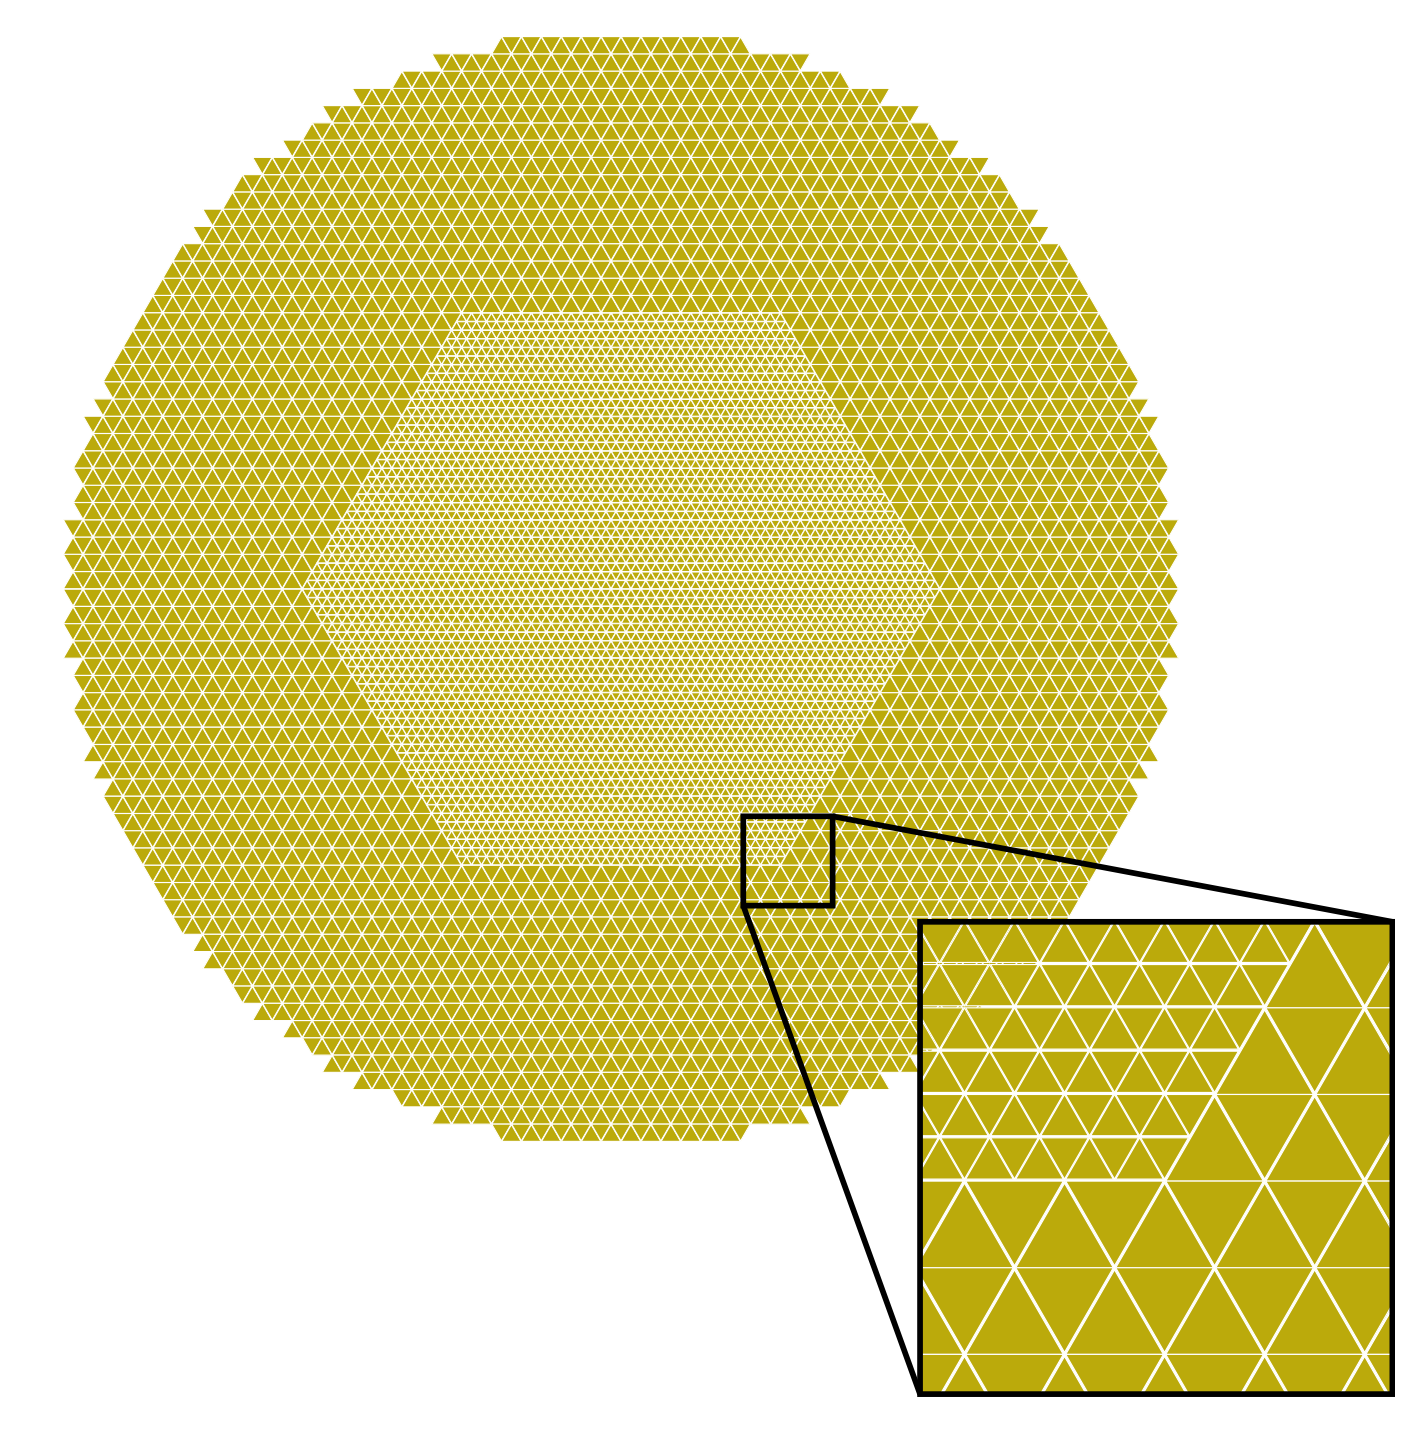
\includegraphics[height=3cm]{../chapters/experimental_background/plots/at_tpc_padplane.png}
		\caption{Detector pad plane of the AT-TPC \footcite{Bradt2017a}}\label{fig:padplane}
	\end{figure}
	Each triangle represents spatial discrete regions of the detector surface. The pad-plane consists of some $10^4$ sensor pads on a circle with $r=29cm$
\end{frame}

\begin{frame}[t]{AT-TPC Data}
	\begin{figure}[t]
		\centering
		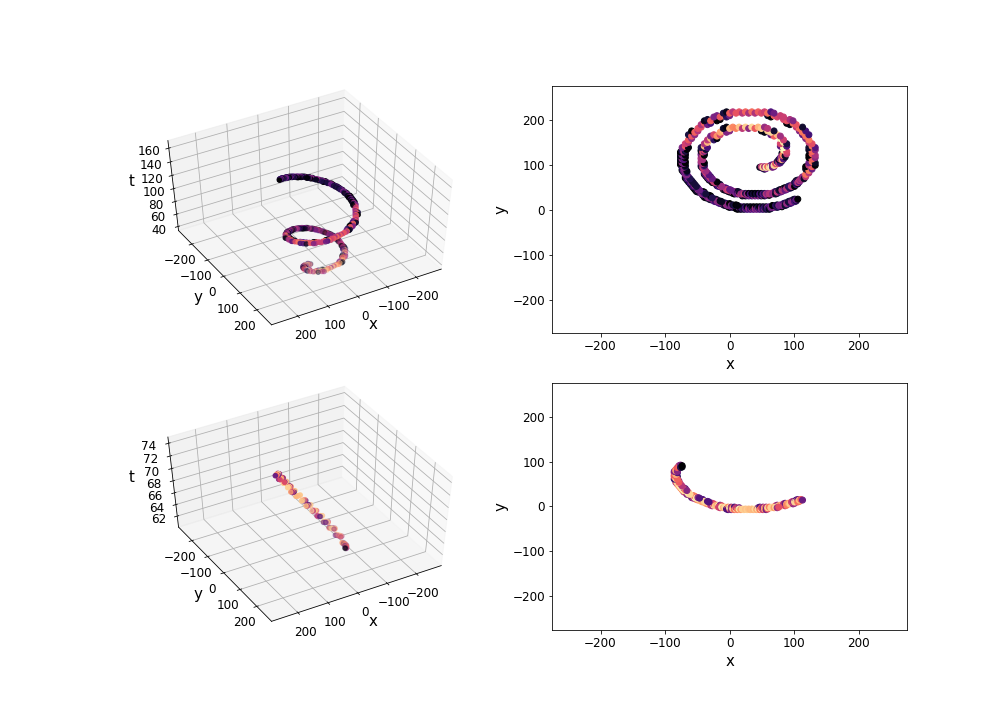
\includegraphics[width=0.8\linewidth]{../chapters/experimental_background/plots/display_eventssimulated.png}
		\caption{Simulated AT-TPC data in an experiment with ${}^{46}$Ar}
		\label{fig:name}
	\end{figure}
\end{frame}

\begin{frame}[t]{AT-TPC Data}
	\begin{figure}
		\subfloat[Unfiltered events from the ${}^{46}$Ar experiment]{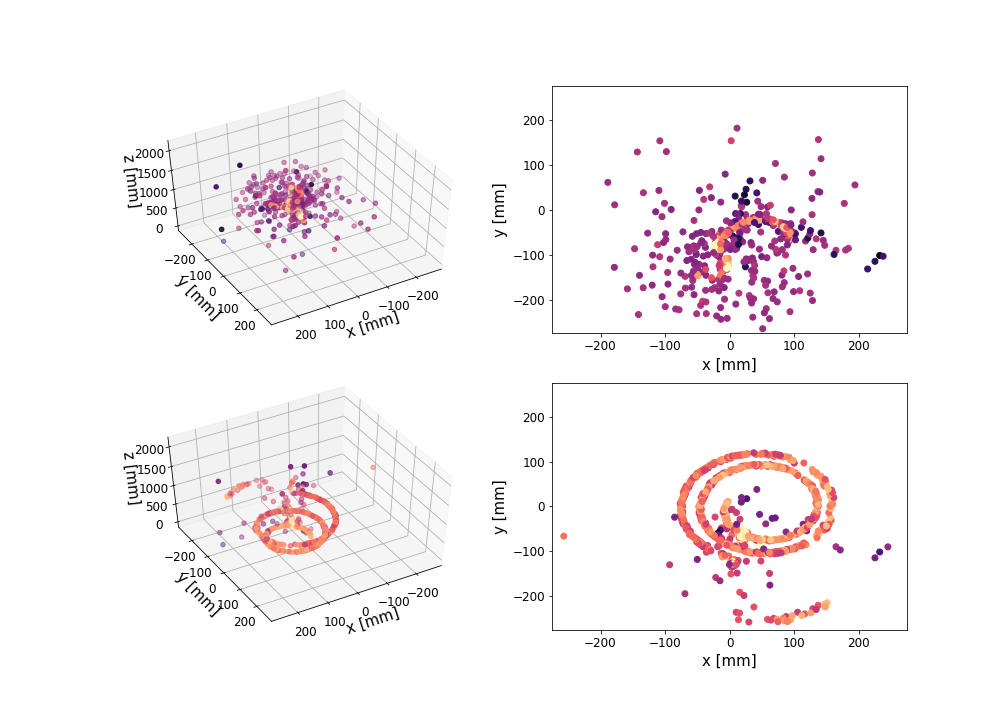
\includegraphics[width=0.4\linewidth]{../chapters/experimental_background/plots/display_eventsfull_.png}}
		\subfloat[Noise-filtered events from the ${}^{46}$Ar experiment]{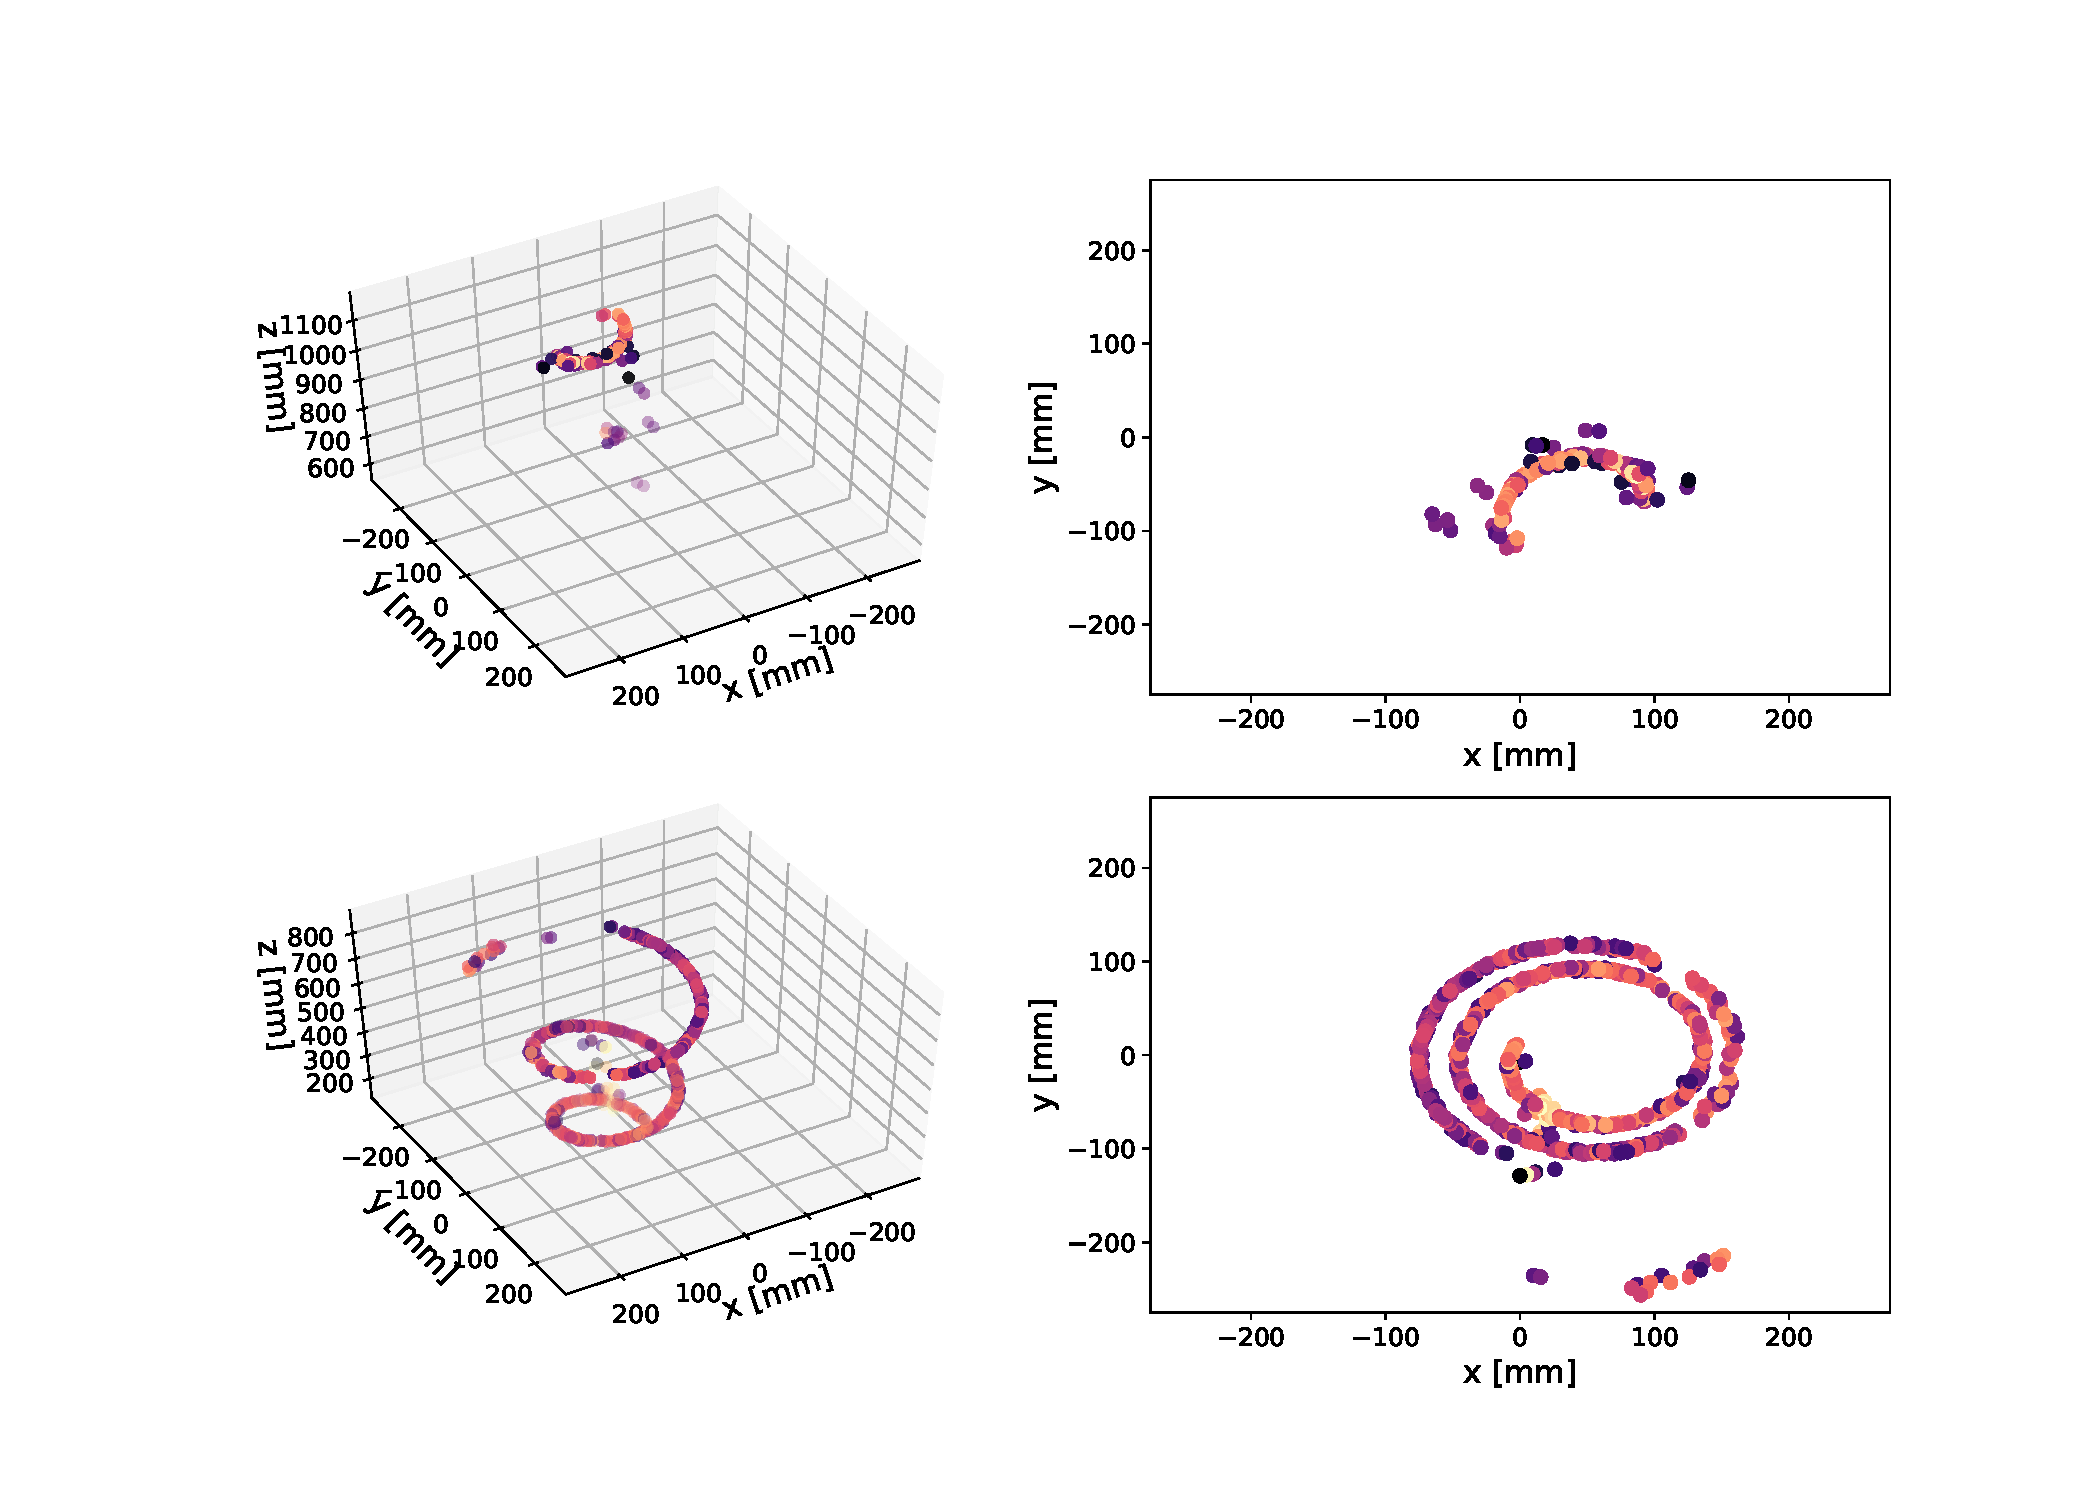
\includegraphics[width=0.5\linewidth]{../chapters/experimental_background/plots/display_eventsclean_.pdf}}
	\end{figure}
	Significant noise levels in the experiment, from unknown sources. Some $60\%$ of the recorded events are from unidentified reactions.
\end{frame}

\begin{frame}[t]{Challenges with the AT-TPC}
	\begin{enumerate}[I]
		\item Expensive integration - for each event a fit is computed.
		\item Assumptions of the integration technique: 
			\begin{enumerate}[(i)]
				\item Each event is fit against parameters of the event of interest,
				\item The integration is sensitive to Noise and Breaks in the tracks.
			\end{enumerate}
		\item In some experiments researchers are unable to identify samples of the positive class of events.
	\end{enumerate}
	The amount of data is also significant: the experiment generates on the order of $10^5$ events per hour running.
	\begin{block}{Idea}
		Solve the problem by training deep neural networks.
	\end{block}
\end{frame}

\begin{frame}[t]{Previous Work}
	\begin{itemize}
		\item Work on applying ML to this data started with a supervised learning project by Kuchera et al.\footcite{Kuchera2019}.
		\item The authors explored a \textit{supervised classification} problem of identifying reactions when ground-truth labels available.
		\item By fine tuning pre-trained networks the authors achieve very impressive performance.
	\end{itemize}
	One of the open questions is then, can we segment the events based on reactions without the ground truth labels?
\end{frame}

\begin{frame}[t]{ML background}
	Machine Learning (ML) is an amorphous set of algorithms for pattern recognition and function approximation. Including models like:
	\begin{enumerate}[I]
		\item Linear Regression
		\item Logistic Regression
		\item Random Forest Classifiers
		\item Genetic Algorithms 
		\item Neural networks
	\end{enumerate}
	And many others...
\end{frame}

\begin{frame}[t]{Why machine learning}
	\begin{enumerate}[I]
		\item Modern computing resources has created a resurgence in ML fostering strong results in other fields.
		\item Very strong results on image-like data. The resurgence brought Convolutional Neural Networks to the forefront.
		\item Agnostic models can be applied very close to source data, possibly avoiding biases.
		\item Broader perspective on what role ML has in physics?
	\end{enumerate}
\end{frame}

\begin{frame}[t]{Deep Learning}
	A branch of machine Learning.

	The premise of Deep Learning is to formulate an approximation to some unknown function $f(\mathbf{x})$ with a model, $\hat{f}$. 

	Some examples of the unknown function, $f(\mathbf{x})$, we would want to approximate are:
	\begin{enumerate}[(a)]
		\item a Hamiltonian of a system 
		\item a function which determines the thermodynamic phase of a system
		\item a function which itentifies dog-species from a picture
	\end{enumerate}
\end{frame}

%\begin{frame}[t]{Deep Learning}
%	Then then model can be tuned with gradient methods, the simplest of which is a steepest descent update: 
%	\begin{equation}
%		\theta_i \leftarrow \theta_i - \eta \frac{\partial \mathcal{C}(\mathbf{x}, f, \hat{f})}{\partial \theta_i},
%	\end{equation}
%	moderated by a \textit{learning rate} $\eta$ to ensure that the steps are small enough.
%
%	The functional $\mathcal{C}$ is the \textit{cost} function for the problem and is commonly a variation of either, the Mean Squared Error: 
%
%	\begin{equation}
%		\mathcal{C}(\mathbf{x}, f, \hat{f}) = \sum (f(\mathbf{x})_i - \hat{f}(\mathbf{x})_i)^2,
%	\end{equation}
%
%	or the Cross Entropy
%
%	\begin{equation}
%		\mathcal{C}(\mathbf{x}, f, \hat{f}) = -\sum f(\mathbf{x})_i \log \hat{f}(\mathbf{x})_i. 
%	\end{equation}
%\end{frame}

\begin{frame}[t]{Deep Learning: Neural Networks}
	\begin{figure}[h]
		\centering
		\includegraphics[width=0.4\linewidth]{../chapters/theory/figures/ann.pdf}
		\caption{A neural network with three input nodes, two hidden nodes, and one output node}
		\label{fig:ann}
	\end{figure}
	Each of the \textit{activations} $a_i$ are computed from the values in the previous layer. 
	The figure illustrates a \textit{forward pass} of the network.
\end{frame}

\begin{frame}[t]{Training Neural Networks}
	\begin{figure}[h]
		\centering
		\includegraphics[width=0.6\linewidth]{../chapters/theory/figures/gd_good.pdf}
		\caption{Gradient descent on a quadratic function}
		\label{fig:gd}
	\end{figure}

	Training neural networks is achieved with first order gradient optimization.
	The function to be optimized is the cost: meaasuring the quality of the current state of the network.
\end{frame}

\begin{frame}[t]{Hazards in Training}
	\begin{figure}[h]
		\centering
		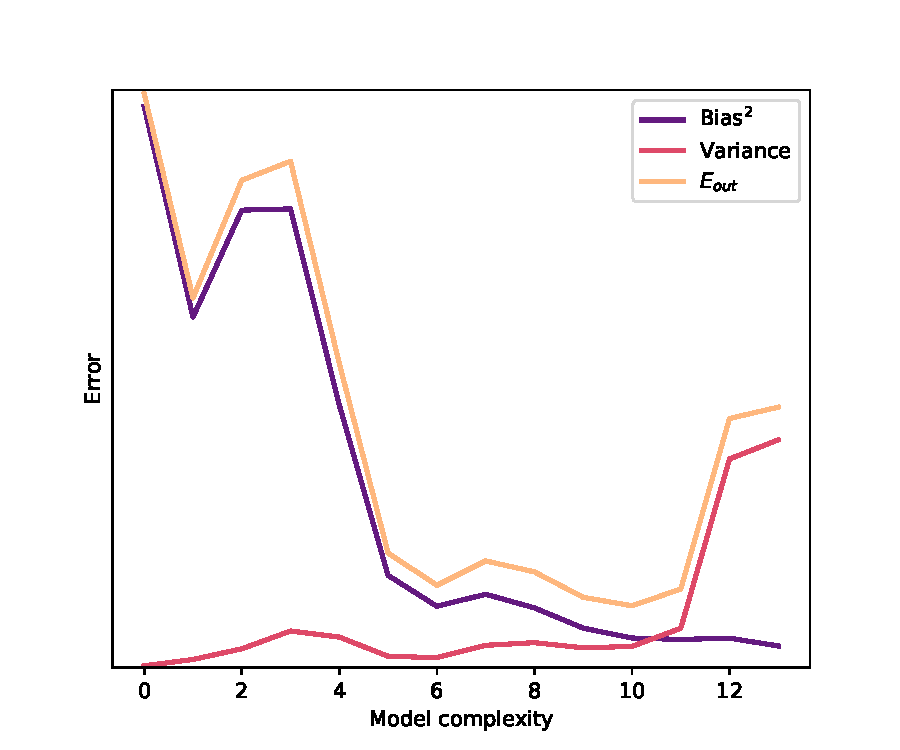
\includegraphics[width=0.55\linewidth]{../chapters/theory/figures/bias_var_degree.pdf}
		\caption{Bias - variance decomposition of the MSE objective with iid. noise. Generalization error is denoted $E_{out}$, and is the sum of the Bias and Variance terms.}
		\label{fig:bv}
	\end{figure}
	The quality of a model is measured by how well it does on data not seen during training, measured by $E_{out}$.
\end{frame}

\begin{frame}[t]{Deep Learning: Network Types}
	\begin{figure}[h]
		\centering
		\subfloat[Convolutional architecture capturing local structures \footcite{Dumoulin2016}]{\includegraphics[width=0.2\textwidth]{../chapters/theory/figures/conv_zeropad_illustration.png}}
		\subfloat[Recurrent architecture for serialized applications \footcite{Jianqiang19}]{\includegraphics[width=0.8\textwidth]{rnn.png}}
	\end{figure}
\end{frame}
\begin{frame}[t]{Autoencoders}
	\begin{itemize}
		\item Recall that we want to separate classes of reaction products
		\item Additionally - we assume that we have access to very little or no ground truth labelled data
	\end{itemize}
	\begin{block}{ Idea }
		Learn the distribution over the events through two nonlinear maps which compress and inflate a representation of the events.
	\end{block}
	\begin{block}{Central Hypothesis}
		If we can create a compressed representation of an event from which we can reconstruct the event - the compression should be informative\footcite{Fertig} of the type of event that occurred.
	\end{block}
\end{frame}

\begin{frame}[t]{Autoencoders}
	\begin{figure}[h]
		\centering
		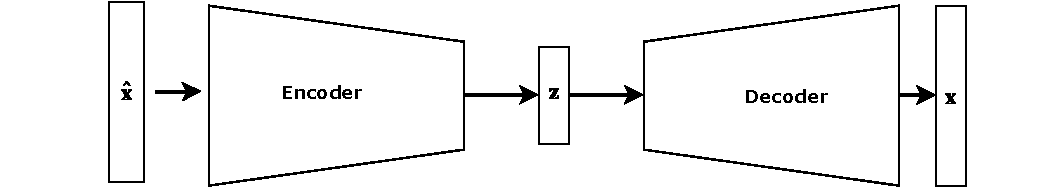
\includegraphics[width=0.8\linewidth]{../chapters/theory/autoencoder/plots/autoencoder.pdf}
		\caption{Autoencoder neural network schematic}%
		\label{fig:autoenc}
	\end{figure}

	An autoencoder is defined by an encoder/decoder pair of neural networks. We construct these such that 
	\begin{align}
		\text{dim}(\mathbf{\hat{x}}) \gg \text{dim}(\mathbf{z}),
	\end{align}

	and with the optimization objective
	\begin{align}
		\mathcal{O} = \text{arg min} || \mathbf{\hat{x}} - \text{Decoder}(\text{Encoder}(\mathbf{\hat{x}}))||_2 ^2.
	\end{align}
\end{frame}

\begin{frame}[t]{Implementing details}
	Models implemented in Python with TensorFlow (TF), a ML framework developed by Google.
	TensorFlow provided a base on which to build complex NN models.
	Code written for this analyis includes 

	\begin{enumerate}[I]
		\item Abstraction for autoencoder networks,
		\item Implementation of variations on the Variational Autoencoder,
		\item Custom class implementations based on the high-level Keras API for deep clustering.
	\end{enumerate}
\end{frame}

\begin{frame}[t]{Experiment}
	\begin{itemize}
		\item We chose to represent the data as 2D projections, neglecting the z-axis.
		\item An autoencoder network is then fit to the events in an end to end manner.
		\item After traing, we extract the compressed (or \textit{latent}) expressions of the data.
		\item With varying amounts of labelled ground-truth data we fit a very simple classifier to the latent expressions
	\end{itemize}
	We wish to construct latent spaces that are as close to trivially separable, and so use a logistic regression classifier.
\end{frame}

\begin{frame}[t]{Results}
	\begin{figure}[h]
		\subfloat[Convolutional autoencoder performance with a naive architecture]{\includegraphics[height=3.5cm]{../chapters/results/classification/plots/ac_n_samples.pdf}}
		\subfloat[Convolutional autoencoder performance using a VGG16 representation representation of the events.]{\includegraphics[height=3.5cm]{../chapters/results/classification/plots/vgg_ac_n_samples.pdf}}
	\end{figure}
	
\end{frame}
\begin{frame}[t]{Clustering}
	\begin{itemize}
		\item We demonstrated that we can construct high quality spaces that are linearly separable
		\item The next step then is a \textit{clustering} task. Can we separate classes without knowing the ground truth labels? 
		\item Clustering, while similar to classification have some principal differences.
	\end{itemize}
	We explored two autoencoder-based clustering algorithms, in addition to ordinary K-means clustering.
\end{frame}

\begin{frame}[t]{K-means clustering}
	\begin{itemize}
		\item Ordinary K-means on the two-dimensional representations would obviously not be productive because of the dimensionality of the problem.
		\item Instead we try to cluster the representation of the events as seen by an image classifying algorithm: VGG16
	\end{itemize}

	With $8e3$ output nodes the VGG16 representation is still very much high dimenisonal, but importantly it is sparse.
\end{frame}

\begin{frame}[t]{K-means results}
	\begin{figure}[h]
		\centering 
		\subfloat{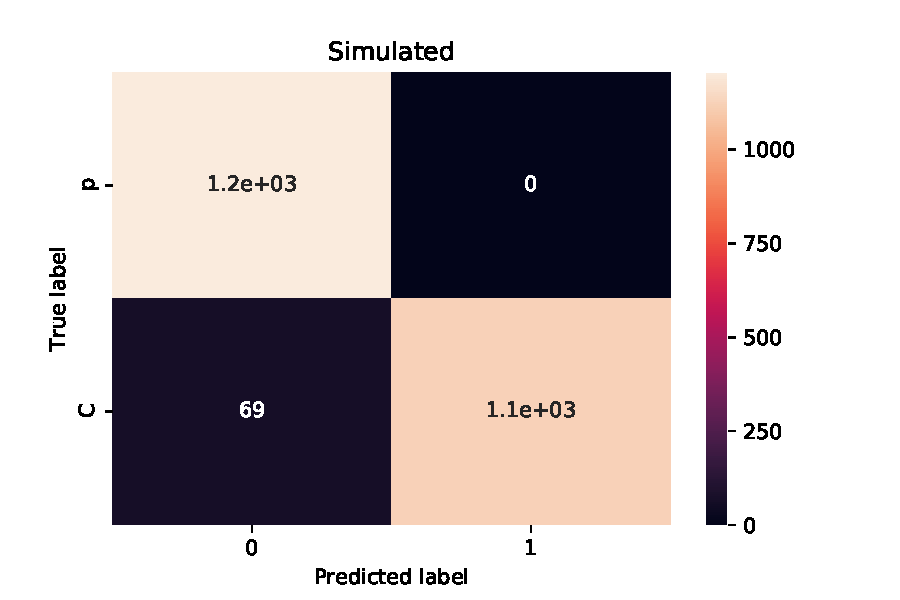
\includegraphics[width=0.3\textwidth]{../chapters/results/clustering/plots/Simulatedvgg_pca_conf_mat.pdf}}
		\subfloat{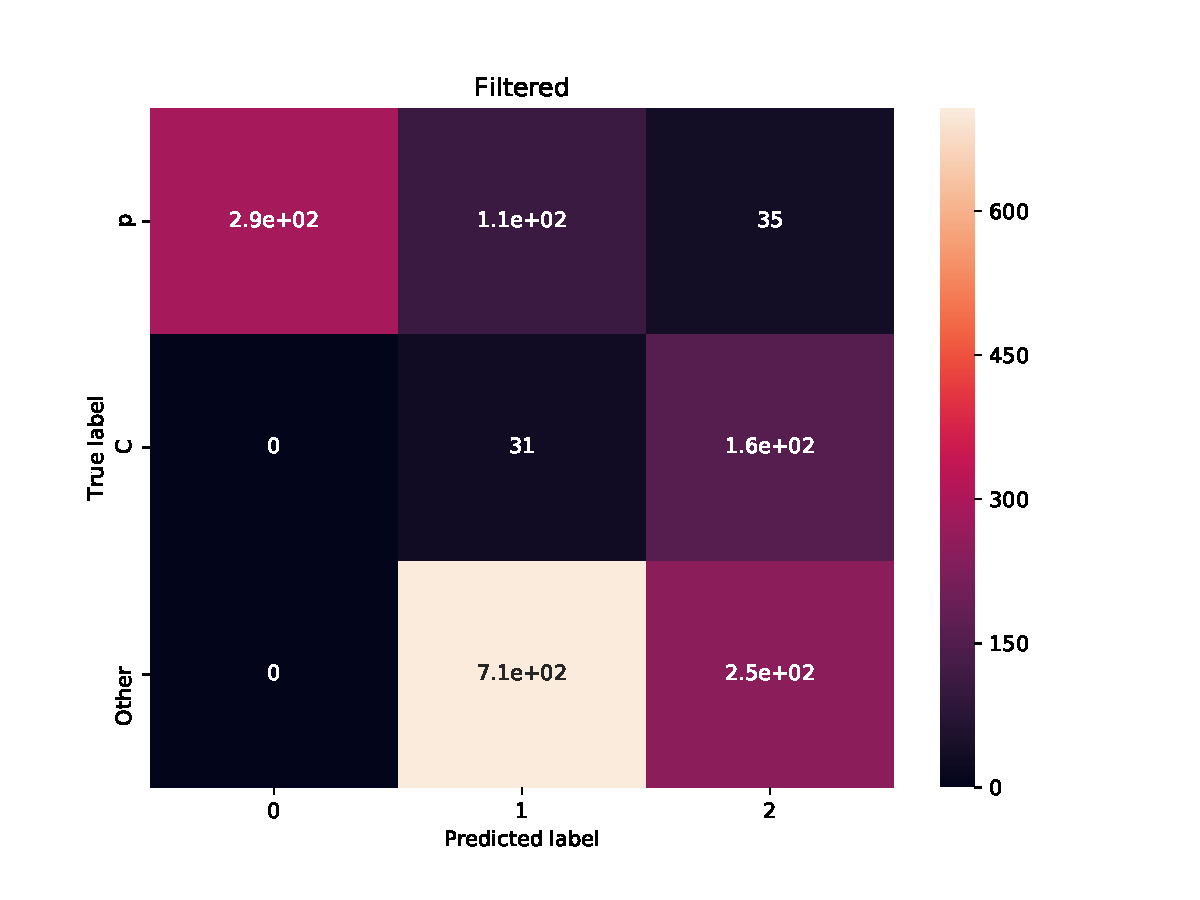
\includegraphics[width=0.3\textwidth]{../chapters/results/clustering/plots/Filteredvgg_pca_conf_mat.pdf}}
		\subfloat{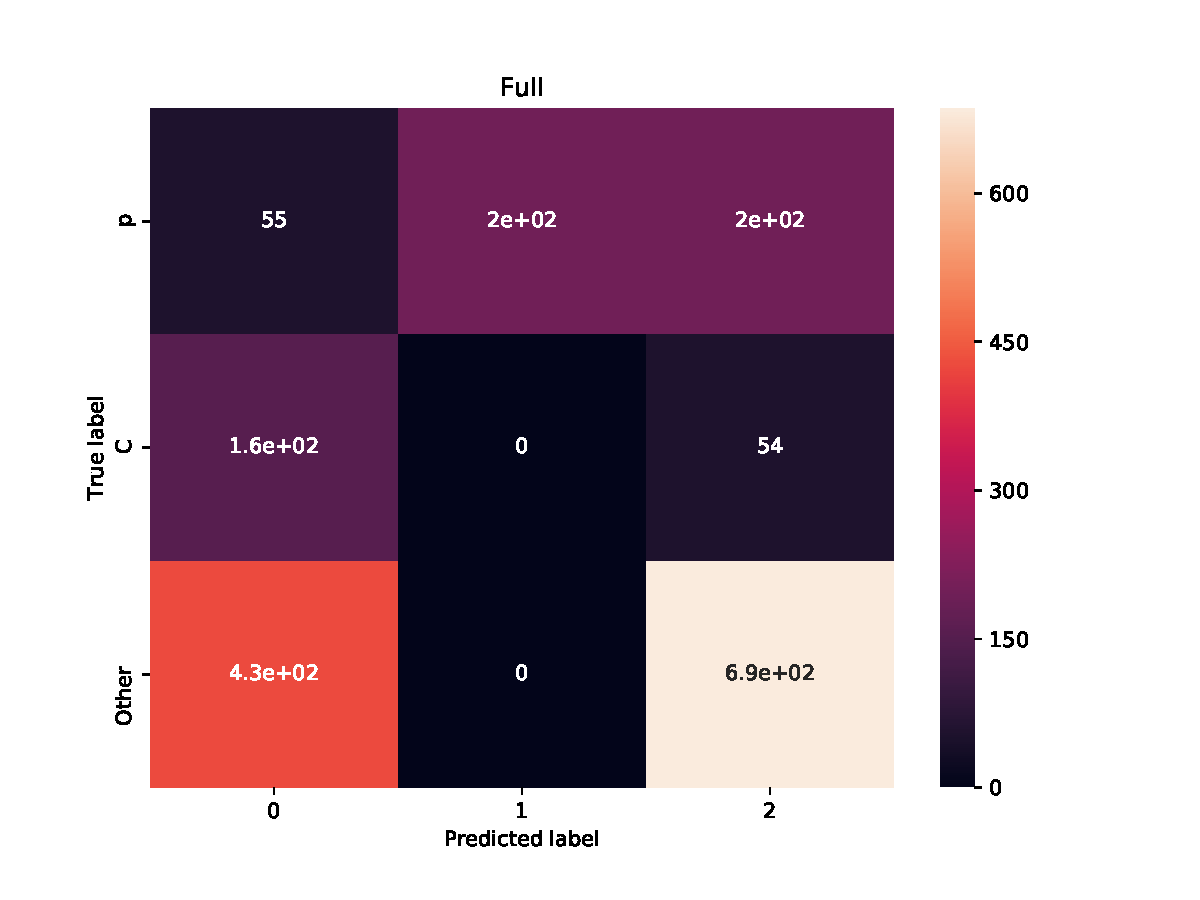
\includegraphics[width=0.3\textwidth]{../chapters/results/clustering/plots/Fullvgg_pca_conf_mat.pdf}}
		\caption{K-means clustering results using the VGG16 representation of the datasets}
	\end{figure}
	Cluster elements for clustering full data 
	\centering 
	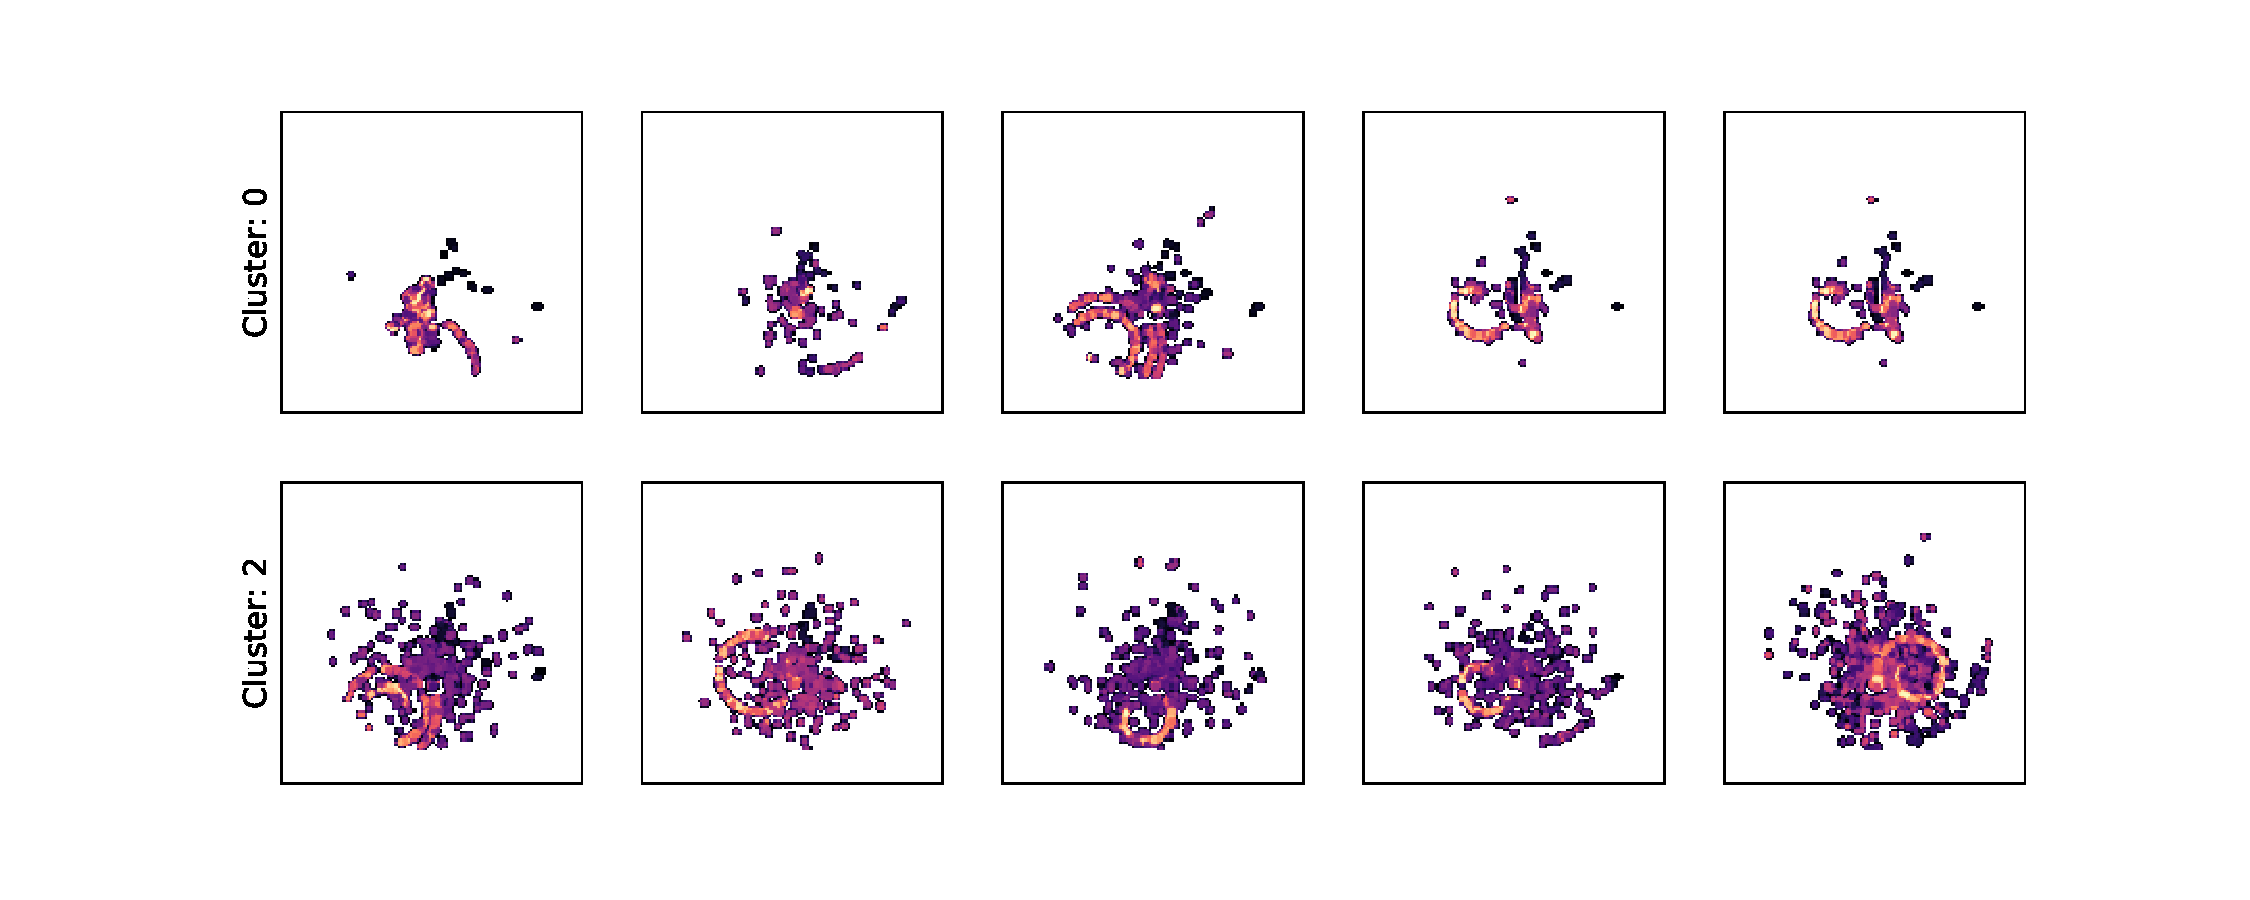
\includegraphics[height=3cm]{../chapters/results/clustering/plots/full_vgg_cluster_repr.pdf}
\end{frame}

\begin{frame}[t]{Mixture of Autoencoders}
	\begin{itemize}
		\item One can also attempt clustering with Autoencoder based algorithms
		\item Niche field with only limited applications (MNIST, Reuters)
	\end{itemize}

	\centering
	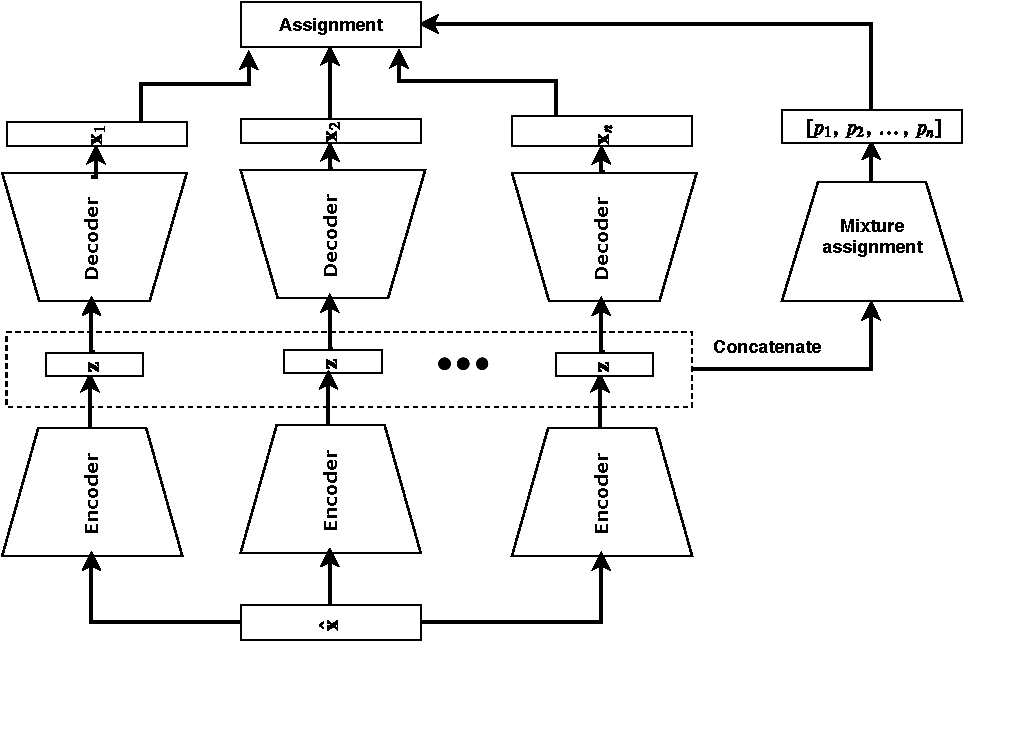
\includegraphics[height=6cm]{../chapters/theory/autoencoder/plots/mixae.pdf}
\end{frame}


\begin{frame}[t]{Deep Clustering Results}
	\centering 
	\begin{figure}[h]
		\subfloat{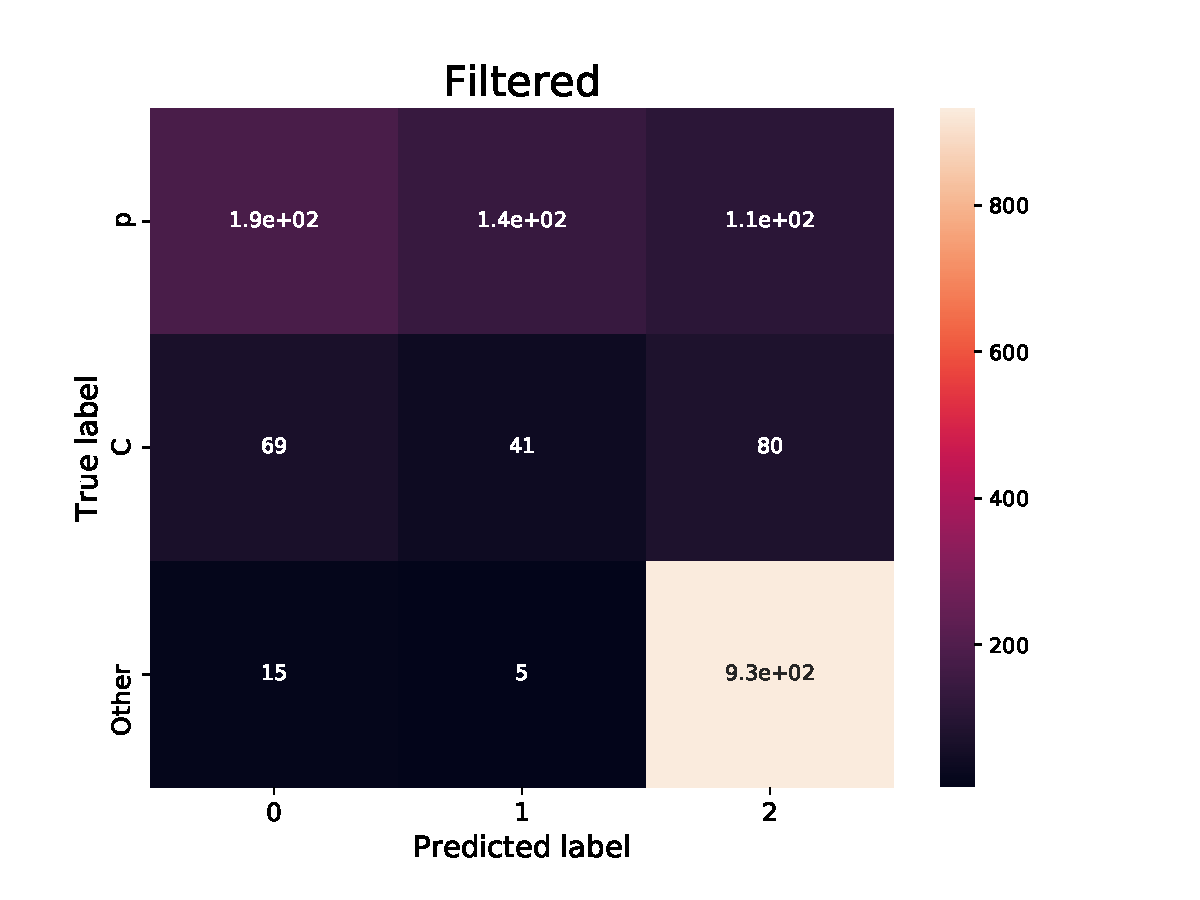
\includegraphics[height=3cm]{../chapters/results/clustering/plots/Filtered_mixae_conf_mat.pdf}}
		\subfloat{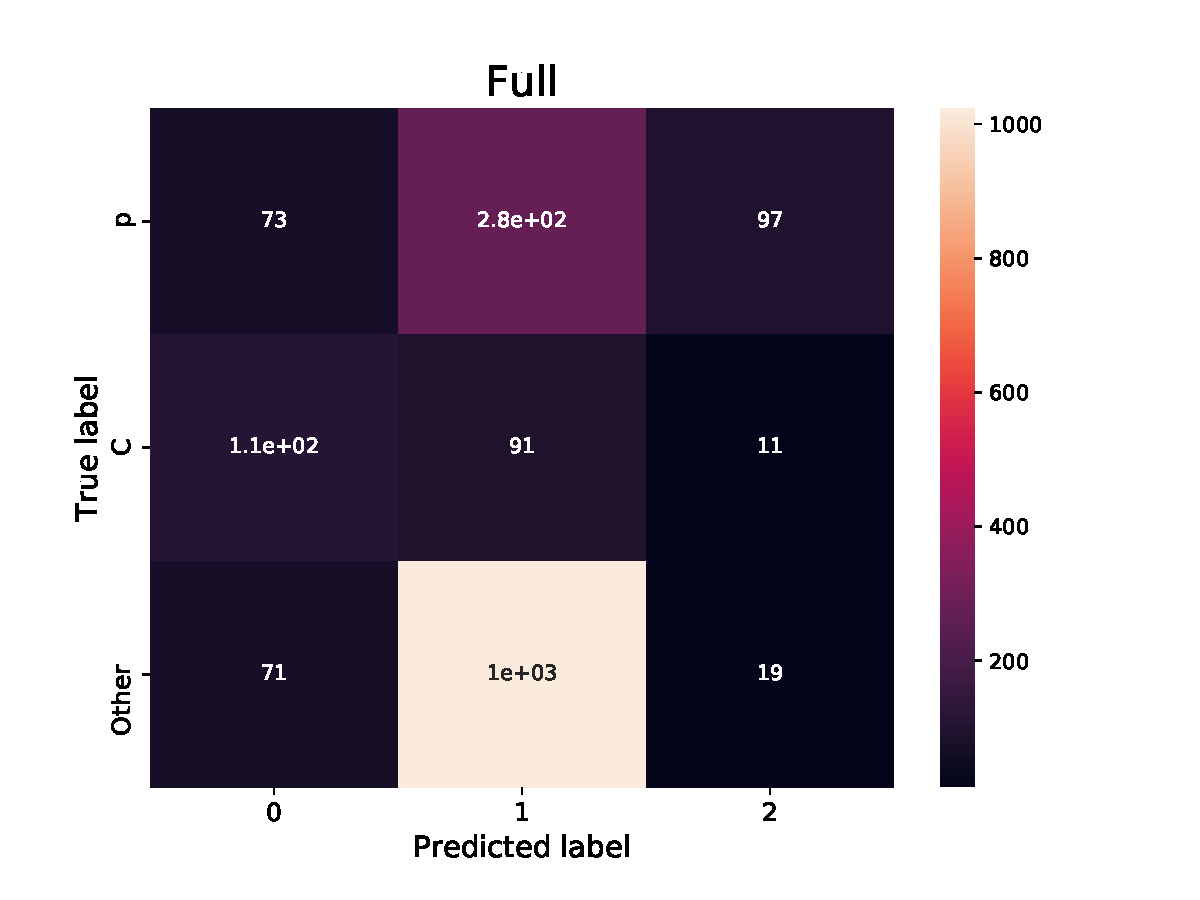
\includegraphics[height=3cm]{../chapters/results/clustering/plots/full_mixae_conf_mat.pdf}}
		\caption{Top-performing mixae results for the real experimental data}
	\end{figure}
	Cluster elements for clustering of full data
	
\includegraphics[height=3cm]{../chapters/results/clustering/plots/real_cluster_repr.pdf}
\end{frame}

\begin{frame}[t]{Summary and Outlook}
	\begin{itemize}
		\item We have shown that Autoencoder models are suitable for both semi-supervised and unsupervised applications.
		\item Autoencoder clustering has a fundamental challenge with issues of stability and convergence. We still need labelled samples to verify.
		\item Including physical parameters increases the quality of the latent space.
	\end{itemize}
	Neural network models clearly have a place in this analyisis going forward: but connecting the anlysis to the physical properties of the system remains a challenge to solve.
\end{frame}
\end{document}
